\documentclass[12pt,a4paper]{article}
\usepackage[a4paper, margin=1in]{geometry}
\usepackage[utf8]{inputenc}
\usepackage[T1]{fontenc}
\usepackage{graphicx}
\usepackage{latexsym}
\usepackage{amsfonts,amssymb,amsmath,amsthm}
\usepackage{multirow}
\usepackage{multicol}
\setlength{\columnsep}{1.5cm}
\usepackage{setspace}
\usepackage{url}
\usepackage{array}
\usepackage{xfrac}
\usepackage{mwe}
\usepackage{tikz}
\usepackage{lmodern}
\usepackage{flowchart}\usetikzlibrary{shapes,arrows,positioning,calc,fit}
\usepackage{graphics}
\usepackage{subfig}
\usepackage{booktabs}
\usepackage{float}
\usepackage{color,soul}
\usepackage[numbers,sort&compress]{natbib}
\usepackage{hyperref}
\usepackage{biblatex}
\addbibresource{References.bib}
\title{Thank You, Next}
\author{Ali M. Campbell\\
Tom E.X. Miller}
\begin{document}
	\maketitle
%	\begin{multicols}{2}
	
	\section*{Abstract}
	
	Understanding interspecific mutualisms is a challenge, because they are among the most widespread species interactions with diverse and dynamic consequences. Depending on the environmental contexts the outcome of an interspecific cooperation can range from parasitic to mutualistic. Most studies focus on a pair of species interacting in a mutualism, however often this is a simplification of the reality. These mutualistic interactions become even more complex when put into the context of a multi-species mutualism, where there are multiple partners interacting with the same focal species. The partners can directly impact the focal species through the interactions, and indirectly impact them through interactions with each other. The cactus \textit{Cylindriopuntia imbricata} forms symbioses with multiple ant species, but each individual plant is able to interact with only one species at a time. Using a long-term data-set, we show that there are differences in the impacts of different ant partners on various vital rates of the cacti across ontogeny.Our results demonstrate the importance of evaluating a mutualism within a community context and suggest that even slight differences of rewards between mutualist partners can help promote fitness of the cacti. 
	
	Each of the ant partners in this system are within the same guild, all offering defense from herbivores, with only one ant species interacting with each individual cactus in a given period of time. Though these ants may offer very similar rewards, they likely differ in some way. Two possible ways they could differ are the fitness boost they offer the focal species or the period of ontogeny in which they offer the greatest fitness boost. Using a long-term data-set, we show that there are differences in the impacts of different ant partners on various vital rates of the cacti across ontogeny. Our results demonstrate the importance of evaluating a mutualism within a community context and suggest that even slight differences of rewards between mutualist partners can help promote fitness of the cacti. 
	
	
	\section*{Context/Introduction}
	\subsection*{Context}
	
	Mutualisms are species interactions in which all involved participants benefit. They are among the most widespread species interactions\cite{Chamberlain2014,Stachowicz2005,BoucherDouglasH.1985} with diverse and dynamic consequences, yet they are still poorly understood. They form a complex foundation to many natural systems which involve both costs and benefits, despite their nature of being beneficial. 
	
	There are benefits of mutualistic interactions, but there are costs as well, some direct and some indirect. Directly, mutualistic partners can sometimes become parasitic, causing harm to the focal mutualist\cite{Bronstein2001a}. More indirectly, these interactions require energy. Within a mutualism, each participant offers rewards and in return receives benefits from their partners. These rewards come in many forms, nectar, protection, habitat, etc., all of which require some investment from the individual\cite{Bronstein2001}. These investments can be seen as the costs of mutualisms, they are traded for the rewards provided by a partner. Because of these trade-offs, there are both costs and benefits to a mutualistic interaction\cite{Bronstein2001,Bronstein2001a}, particularly as the mutualism becomes more complex in the context of its environment. 
	
	Mutualistic interactions can occur simply between two species, a pairwise mutualism, or between a group of species, a multi-species mutualism\cite{Stanton2013}. Pairwise mutualisms may provide benefits of efficiency in the context of mutualisms, but they are not a good investment due to temporal and spatial variation\cite{Waser1996}. Despite this, pairwise mutualisms are historically well studied, with most mutualism papers being focused on pairwise interactions. These studies are often used to predict outcomes of mutualistic interaction, which may underestimate the combined impacts of multiple partners on the focal mutualist\cite{Stanton2013,Palmer2010}. Pairwise interactions do not always indicate what the net interaction will be within a multi-species context\cite{Chamberlain2014,Song2020}. When many species are included, variation between partners can occur in functional benefit, lifespan, and competitive rankings, among other factors\cite{Stanton2013}. This difference is because in addition to the expected direct benefits of interactions, they can also indirectly impact the focal mutualist through other partner interactions. One reason for this lack of predictability is that interactions between partners changes the relationship with the focal mutualist\cite{Afkhami2014}.  Often the partners interact with each other, either increasing their performances, with extra rewards, or decreasing them, often by fighting\cite{Boucher1982}. This means predicting the rewards of a multi-species mutualism is very difficult. 
	
	
	Multi-species mutualisms are not always additive: In theory if multiple partners can all form pairwise mutualisms with a focal species, in a multi-species mutualism one would expect more benefits for the focal partner than in any one pairwise scenario. The reality is much less predictable\cite{Stanton2013,Palmer2010,Song2020}. The rewards can be as simple as the sum of all pairwise rewards, aka. additivity, they can be increased beyond the sum of all pairwise rewards, synergy, or they can be reduced below the sum of pairwise rewards, sub-additivity. Specifically, it can often change the quality of benefits. 
	
	Sometimes a partner can confer benefits on the focal mutualist in a pairwise interaction but be a neutral or even antagonistic interactor in a multi-species interaction as partners can vary in quality\cite{Afkhami2014}. Some mutualists are of so low a quality that they are known as freeloaders or cheaters\cite{Song2020,West2007,Frederickson2013} because they return very little benefit, possibly going as far as to be a cost to the focal mutualist in exchange for the benefits they receive. This change in quality of partners is often due to competition between the partners\cite{Amarasekare2003}. Some partners reduce in quality so drastically that they become antagonistic towards the focal mutualist in these relationships\cite{Afkhami2014,Frederickson2013,Bronstein1994}. Despite the potential to reduce fitness of the focal mutualist they often remain a partner within the mutualism\cite{Jones2015}. 
	
    There are several underlying mechanisms which promote partner diversity that may shed some light on this; specifically, sampling effect,portfolio effect, and complementarity, three branches of biodiversity ecosystem function theory\cite{Batstone2018,Hooper2005}. 
    
    Sampling effect states that if partners vary in quality, then a more diverse sample of the partner community may be more likely to include the most beneficial one\cite{Afkhami2014}. Particularly, this means that increased diversity of partners means increased probability that some of the partners will be highly beneficial. The fitness of a multi-species mutualistic population experiencing sampling effect will be equal to the fitness of the same population if they interacted only with their strongest partner. 
    
    Complementarity states that each partner may account for some part of the benefits, but each has different functional pathways, which together can aid in a broader benefit\cite{Winfree2020}. This means that in populations where there is sufficient interaction with the diverse partners there is likely to be increased rewards and fitness. The fitness of a multi-species mutualistic population experiencing complementarity is likely to be higher than that of any pairwise mutualistic population. 
    
    Portfolio effect states that each partner is the best under a different set of conditions, meaning across all conditions, meaning there is likely to be an increase in potential benefits\cite{Winfree2020}. Thus, in populations experiencing highly diverse conditions, diverse partners are likely to increase the rewards and fitness of the focal mutualist. The fitness of a multi-species mutualistic population experiencing portfolio effect is likely to have a different strongest partner under different conditions, such as year to year, and will experience similar fitness as they would in a pairwise mutualism with their best partner under any condition.  
    
    These biodiversity ecosystem functions are three which can be used to explain the diversity of mutualistic relationships in nature\cite{Afkhami2014}. If a system benefits from the existence of multiple partners, one of these functions may be at play. Within the section of mutualistic interaction which have multiple partners, there are many different classifications. One type of mutualism that is historically well documented is the interaction between ants and plants\cite{Boege2005,Barton2010}. These interactions can take many forms, including pollination, defense, dispersal, etc\cite{Bronstein2006}. This paper focuses on defensive ant-plant mutualisms. These often involve long-lived plants providing extra-floral nectar and/or habitats to ants which in turn defend them from herbivores\cite{Bronstein1998}.  These are very common interactions and have provided many opportunities for empirical studies of mutualisms. However, many of these studies have been pairwise rather than investigating the impacts that multiple partners may have on the costs and benefits of a system. 
    
    This study focuses on the long lived, faculative \textit{Cylindriopuntia imbricata} (Cholla cacti) and its ant mutualists. The cacti interact with several ant partners, \textit{Crematogaster opuntiae} (\textit{Crem.}) and \textit{Liometopum apiculatum} (\textit{Liom.}) are the most common partners though there are a number of other rarer ant partners, which visit these cacti in smaller population sizes. The ant partners all provide defense to the cacti from predators in return for exclusive interaction with the plant to take the extra-floral nectar, meaning they are considered to be within one guild. Predators of the cholla include insect herbivores and seed predators, which influence the reproductive output of the cacti. Though many multi-species mutualisms result in both costs and benefits, it has been shown that the relationship between these cacti and ants does not result in any major costs for the cacti\cite{Miller2007}. However, there are still some small costs which could influence the optimal set of partners. This is part of what we will be analyzing in this paper.
    
    Though all the ants associated with the Cholla are within one guild, they may not all be equal, meaning the impacts on the Cholla are complex. In this study, we will answer a number of questions: 
    \begin{enumerate}
        \item Do the Cholla cacti benefit from the multi-species mutualism with multiple ant partners?
        \item What combination of, or individual, ant(s) result in the highest fitness for the Cholla cacti?
        \item Is there evidence of sampling effect, complementarity, or portfolio effect to encourage the current multi-species state of the mutualism?
    \end{enumerate}
    
    In order to answer these questions, I am constructing an Integral Projection Model (IPM) to calculate the fitness of the Cholla cacti under different conditions. I will be able to quantitatively estimate the fitness of the cholla population if they were to interact with any combination of ant partners, allowing me to determine the best combination of partners. Similar approaches have been used to assess the individual qualities of multiple partners\cite{Palmer2010} but not to determine the optimal combination of partners in a multi-species mutualism. 
    
    We hypothesize that the cacti will experience the highest fitness when interacting with all partners observed in the field, meaning the current mutualism is the optimal outcome. We also hypothesize that complementarity and sampling effect will play roles in encouraging this diverse mutualism. 	
	
	\section*{Methods}
		\subsection*{Study System}
    To determine how interactions with multiple partners impacts the cacti over time, we have monitored a population of Cholla cacti annually since 2004, this is still ongoing. This study was conducted in the Los Pinos mountains, a small mountain chain located on the Sevilleta National Wildlife Refuge, a Long-term Ecological Research (LTER) site in central New Mexico. The tree cholla cacti are common in high Chihuahuan desert habitats, with their native range spanning the southwestern USA *** Benson 1982***. These arborescent cacti produce new cylindrical segments every year which develop either into fruits which produce seeds or into vegetative segments with large spine which increase the size of the cactus ***Miller, Tenhumberg & Louda 2008***. In central New Mexico, vegetative growth occurs from May -- August.
	
	The cholla cacti secrete extra-floral nectar (EFN) from glands on young vegetative segments and reproductive segments. This extra-floral nectar varies in chemical makeup across the lifespan of the cactus *** Miller ??***. 
	At the Sevilleta, the cacti are visited by multiple species of ground-nesting ants, \textit{Crematogaster opuntiae}, \textit{Liometopum apiculatum}, and many other species which occur at small frequencies. These ants are attracted to the EFN and in return fight off the seed predators which also visit the cacti. These ants never co-occur on the same plant, instead competing for plant services. Over the lifetime of the cacti each plant interacts with multiple partners as they tend to switch out season to season.
	
	There are a variety of insect herbivores and seed predators which attack the cacti, focusing either on the vegetative segments and the reproductive segments. There are a number of insects which occur commonly on these cacti at the Sevilleta. These include the weevil, the NP, and the *** (I think there is a moth as well?). The weevil feeds on ***. The NP feeds on ***. Finally, the moth?? feeds on ***. All of these predators can have significant impacts on the fitness of both individual cacti and the population. *** Miller 2009***. 
	
	The data collected on these cacti are from an 18-year data-set. There are 8 30 $\times$ 30 meter plots from which this data is taken. Each plot is surveyed, and each plant within each plot is tagged and logged each year. For every plant we take data on their survival, size, ant state, herbivore presence, flowering data, and seed data. This allows us to track the progression of individual plants across many years. The length of this data-set 
	
	\subsection*{Statistical Modeling}
	To understand the impacts of multiple species interactions on the cacti populations, we constructed bayesian demographic models of many vital rates. With these models, we were able to ask (i) Do the impacts of ant presence on cacti fitness differ across ant species? (ii) What are the probabilities of an individual cactus interacting with each ant species?. 
	
	The vital rates of the cacti considered in this model include survival rate, growth rate, reproductive state, floral abortion rate, seed production, and germination. We fit generalized linear mixed effects models in a heirarchical Bayesian framework to quantify each of the vital rates. Each model takes the data from year \textit{t} and estimates the values in year \textit{t+1}. This allows us to predict a vital rate for any plant with a given set of characteristics, such as size and ant state. 
	\vspace{1cm}
	
	
	
	\subsection*{Demographic Modeling}
	
	The statistical models described above parameterize the Integral Projection Model (IPM) that we used to estimate population growth under various partner conditions.  This model was used to estimate the growth rate of the cactus population, effectively a quantitative measure of the fitness of the population. The fitness was estimated under the range of all different conditions, no ants present, one ant species present, two ant species present, all ant species present. These allow us to compare the fitness of the cacti under no mutualistic interactions, pairwise mutualisms, and various multi-species mutualisms to show which case results in the highest fitness for the cacti. Following previous studies, we modeled the life cycle of \textit{C. imbracata} using continuously size-structured plants,$n_i(x)$, and two discrete seed banks ($\beta_{1,t}$ and $\beta_{2,t}$) corresponding to 1 and 2-year old seeds.
$$
B_{1, t+1} = \kappa \delta \sum_{i}^{4} \int_L^U P(x) A_i(x) F(x)n_i(x) dx \\
$$
$$
B_{2,t+1} =  (1 - \gamma_1)B_{1,t}\\
$$

    The functions $P$, $F$, and $A$ give the probability of flowering, the number of flowerbuds produced, and the proportion of flowerbuds which will create seeds. Each of these functions, estimated by a Bayesian model calculates these values for an $x$-sized plant in year $t$. The proportion of flowerbuds which will produce seeds ($A$) is also dependent on the ant species present on the plant $i$ in year $t$. The integral is multiplied by the number of seeds per fruit ($\kappa$) and the probability of seed dispersal/survival ($\delta$) to give the number of seeds that enter the 1-year old seed bank. Parameters $U$ and $L$ are the upper and lower  bounds, respectively, of the plant size distribution. Plants can recruit out of the 1-year seed bank with the probability of $\gamma_1$ or transition to the 2-year seed bank with a probability of $1 - \gamma_1$. Seeds in the 2-year seed bank are assumed to either germinate with a probability of $\gamma_2$ or die. 
    
    The size dynamics of the plants are given by:

$$
n(y,i)_{t+1} = (\gamma_1 B_{1,t} + \gamma_2 B_{2,t}) \eta(y) \omega \beta_i  + \\
$$
$$
\sum_{j}^{4} \int_L^U S_j(x) G_j(y,x) \tau_{ij}(x) n_j(x) dx \\
$$

    The final equation gives the size of the \textit{C. imbracata} population $n$ in year $t+1$ based on the vital rates and size $n$ of the population in year $t$. The first term gives the recruitment from 1 and 2-year seedbanks to size $y$. $\eta(y)$ gives the seedling size distribution, which is assumed to be normally distributed, and $\omega$ gives the proportion of seedlings which survive from germination (late summer) to the census (May). The second term gives the changes in the population of the cacti which are not recruits. The functions $S$ and $G$ give the probabilities of surviving from year $t$ to $t+1$ and growing to size $y$ from year $t$ to year $t+1$, respectively. Each depends on the size $x$ in year $t$ and the ant state $j$ in year $t+1$. Finally, $\tau_{ij}$ is the probability of a cactus which is size $x$ with ant partner $i$ in year $t$ being tended by ant partner $j$ in year $t+1$. 
    
    \subsection*{Model analysis}
    
    

	\section*{Results}
	\subsection*{Vital Rates}
	
	We used field data on cholla cacti to evaluate the differing impacts that the ant mutualism has on the fitness of the cacti. The fitness can be broken down into a number of vital rate components, including survival, growth, probability of flowering, number of fruits and seeds produced, etc. called vital rates. We found that many of these vital rates differ in the presence of different ant species. 
	

	\begin{figure}[!ht]
	\centering
	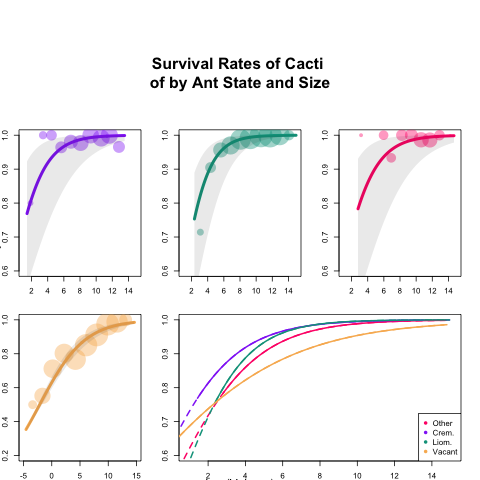
\includegraphics[width = 0.85\linewidth]{Figures/surv_panels_cropped.png}
	\caption{Probability of cactus survival from year t to year t+1 when tended by (a) \textit{Crem.} (Purple), (b) \textit{Liom.} (Teal), (c) ants in the other category (Pink), or (d) no ants (Yellow). Panels (a-d) show the best-fit line estimating the survival probabilities of cacti, with a grey area representing the uncertainty, and circles representing the actual data (scaled to represent number of observations). (e) shows the best-fit probabilities of survival of different-sized cacti with all ant partners.}
	\label{fig:surv}
	\end{figure}

	The first vital rate we analyzed was the survival of the cacti. As you can see in Figure \ref{fig:surv}, the survival rate of cacti vary significantly across their lifetimes as they grow. Young (small) cacti have relatively low survival rates, near $30\%$ while the older mature cacti have much higher survival rates, near $100\%$. This means cacti are at their most vulnerable to death when they are young. The survival rates differ with more than just the size of the cacti, the ant species present on the cactus is also important. 
	
	There are no very small cacti tended by ant partners because they do not produce EFN. This is reflected in Figure \ref{fig:surv} where only the vacant data (yellow) in panel (d) extends to the smallest sizes. Once cacti reach a size large enough to attract ant partners with EFN, the cacti which are partnered with \textit{Crem.} have the highest survival rates compared to all other cacti. When the cacti reach their larger sizes, the partnered plants all reach a nearly $100\%$ survival rate while plants with no partners have a slightly lower survival rate for all large cacti. This result indicates that \textit{Crem.} tended plants may have an advantage, when they are relatively small, over other cacti. 
	
	The next vital rate we analyzed was the viability rate of the cacti, the proportion of fruits produced which are viable for reproduction. It is clear from Figure \ref{fig:viab} that the cacti tended by \textit{Liom.} ants experience significantly higher proportions of viable fruits. This result aligns with much of the literature which shows that \textit{Liom.} are more aggressive against herbivores and seed predators, therefore are very high quality defenders. This high-quality defense is imperative for high viability rates on reproducing cacti which are likely to attract many antagonists due to the quality of their EFN. 
	
	
	\begin{figure}[!ht]
	    \centering
	    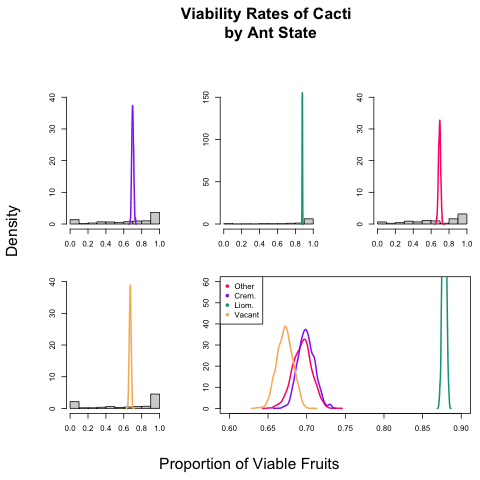
\includegraphics{Figures/viab_hist.png}
	    \caption{Proportion of viable fruits produced by a cactus in year t+1 when tended in year t by (a) \textit{Crem.} (Purple), (b) \textit{Liom.} (Teal), (c) ants in the other category (Pink), or (d) no ants (Yellow). Each panel (a-d) shows a histogram of the actual data overlayed with a density distribution of the predicted viability rate of the cacti. Panel (e) shows the predicted distributions of viability rates separated by ant species.}
	    \label{fig:viab}
	\end{figure}
	
	A third vital rate considered in this paper is the growth rate. Cacti who are attacked by herbivores are likely to lose sections of their growth, leading to a lower, or even negative, growth rate. In Figure \ref{fig:grow} you can clearly see that untended plants are the only cacti which experience a negative growth rate at any size. This again aligns with expectations that tended cacti are being defended from herbivores and are therefore unlikely to lose enough vegetation to result in a negative growth rate. 
	
	\begin{figure}[!ht]
	    \centering
	    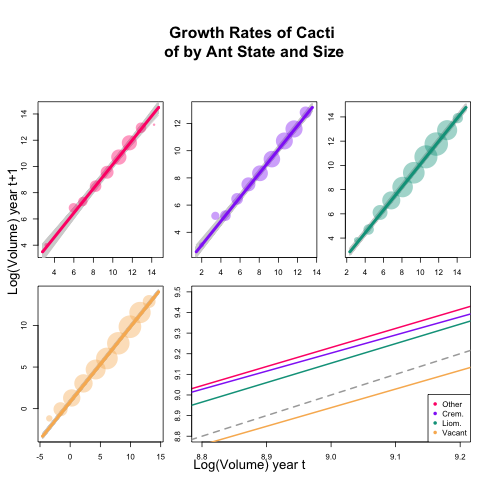
\includegraphics{Figures/grow_panel.png}
	    \caption{The size of a cactus in year t+1 given a previous size in year t and being tended by (a) \textit{Crem.} (Purple), (b) \textit{Liom.} (Teal), (c) ants in the other category (Pink), or (d) no ants (Yellow). Each panel (a-d) shows a best-fit prediction of the future size based on the previous size, the uncertainty in grey surrounding the best-fit, and the actual data in (circles scaled to represent the number of observations). Panel (e) shows all best-fit lines together in the same colors as above and a line (grey, dashed) above which plants are growing (have a positive growth rate) and below which plants have a negative growth rate.}
	    \label{fig:grow}
	\end{figure}
	
	\begin{figure}[!ht]
	    \centering
	    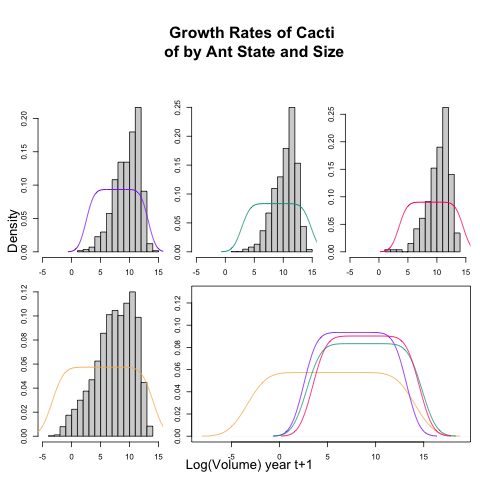
\includegraphics{Figures/grow_dist_panel2.png}
	    \caption{The size of a cactus in year t+1 given a previous size in year t and being tended by (a) \textit{Crem.} (Purple), (b) \textit{Liom.} (Teal), (c) ants in the other category (Pink), or (d) no ants (Yellow). Each panel (a-d) shows a distribution of the predicted future size based on the previous sizeand a histogram of the actual data. Panel (e) shows all predicted distributions together in the same colors as above.}
	    \label{fig:grow2}
	\end{figure}
	
	\subsection*{Ant Transition Rates}
	
	In addition to the vital rates of the cacti, we also analyzed the transition rates from one ant partner to another across years. 

	\begin{table}[]
	    \centering
	    \begin{tabular}{|p{0.25 \linewidth}   |p{0.25 \linewidth}|p{0.25 \linewidth}|}
	    \hline
	        \textbf{Ant States Possible} & \textbf{Growth Rate ($\frac{n_{t+1}}{n_t}$)} & \textbf{Population $\lambda$}\\
	        \hline
	        No ants & &\\
	        \hline
	        \textit{Liom.} & & \\
	        \hline
	        \textit{Crem.}  & & \\
	        \hline
	        Other & & \\
	        \hline
	        \textit{Liom.} \& \textit{Crem.} & & \\
	        \hline
	        \textit{Liom.} \& Other & & \\
	        \hline 
	        \textit{Crem.} \& Other & & \\
	        \hline
	        \textit{Liom.}, \textit{Crem.} \& Other & & \\
	        \hline
	    \end{tabular}
	    \caption{Caption}
	    \label{tab:table_sims}
	\end{table}
%	\begin{multicols}{2}
	
	\section*{Discussion}
	
     There is a constant tension within life cycles between energy and resource allocation. Individuals often have the ability to either put significant resources towards one process or split their resources between multiple. Full energy allocation to one process generally means better results, but splitting resources is a form of bet hedging ***. The cacti studied here experience a certain tension between their many vital rates, particularly growth and reproduction because each year they produce new floral buds and new vegetative growth. Small plants rarely put out flowers and instead focus on growth, but larger plants must choose each year. The analyses of the individual vital rates indicate that different ant species may protect different processes better than others. In particular \textit{Crem.} may offer advantages to smaller plants by protecting their new vegetation well. This is seen in the higher survival rates and growth rates of small and medium cacti with \textit{Crem.} tenders in Figure \ref{fig:grow} and Figure \ref{fig:surv}. \textit{Liom.} ants alternatively may protect reproductive focus more than other partners. The \textit{Crem.} tended plants however, have lower viability rates than any other ant tended plants, indicating they do not protect flowers well from herbivores(Figure \ref{fig:viab}). This is seen in Figure \ref{fig:viab} where it is shown that plants tended by \textit{Liom.} have the highest viability rates of their flowers, resulting in higher pollination rates. Larger plants are also less likely to lose branches when they are tended by \textit{Liom.} (Figure \ref{fig:grow}), keeping them healthy and more able to generate new plants. Each of these ants individually offer both benefits and drawbacks but considered together may indicate complementarity across ontogeny. 
     
%	\end{multicols}

\end{document}

\typeout{\bibliography{References.bib}}